\section{Capítulo 1}
\subsection{Introducción al trabajo}
 
\begin{frame}
\frametitle{Tetris}

Tetris es uno de los videojuegos más conocidos con más de 170 millones de copias vendidas.

\begin{figure}
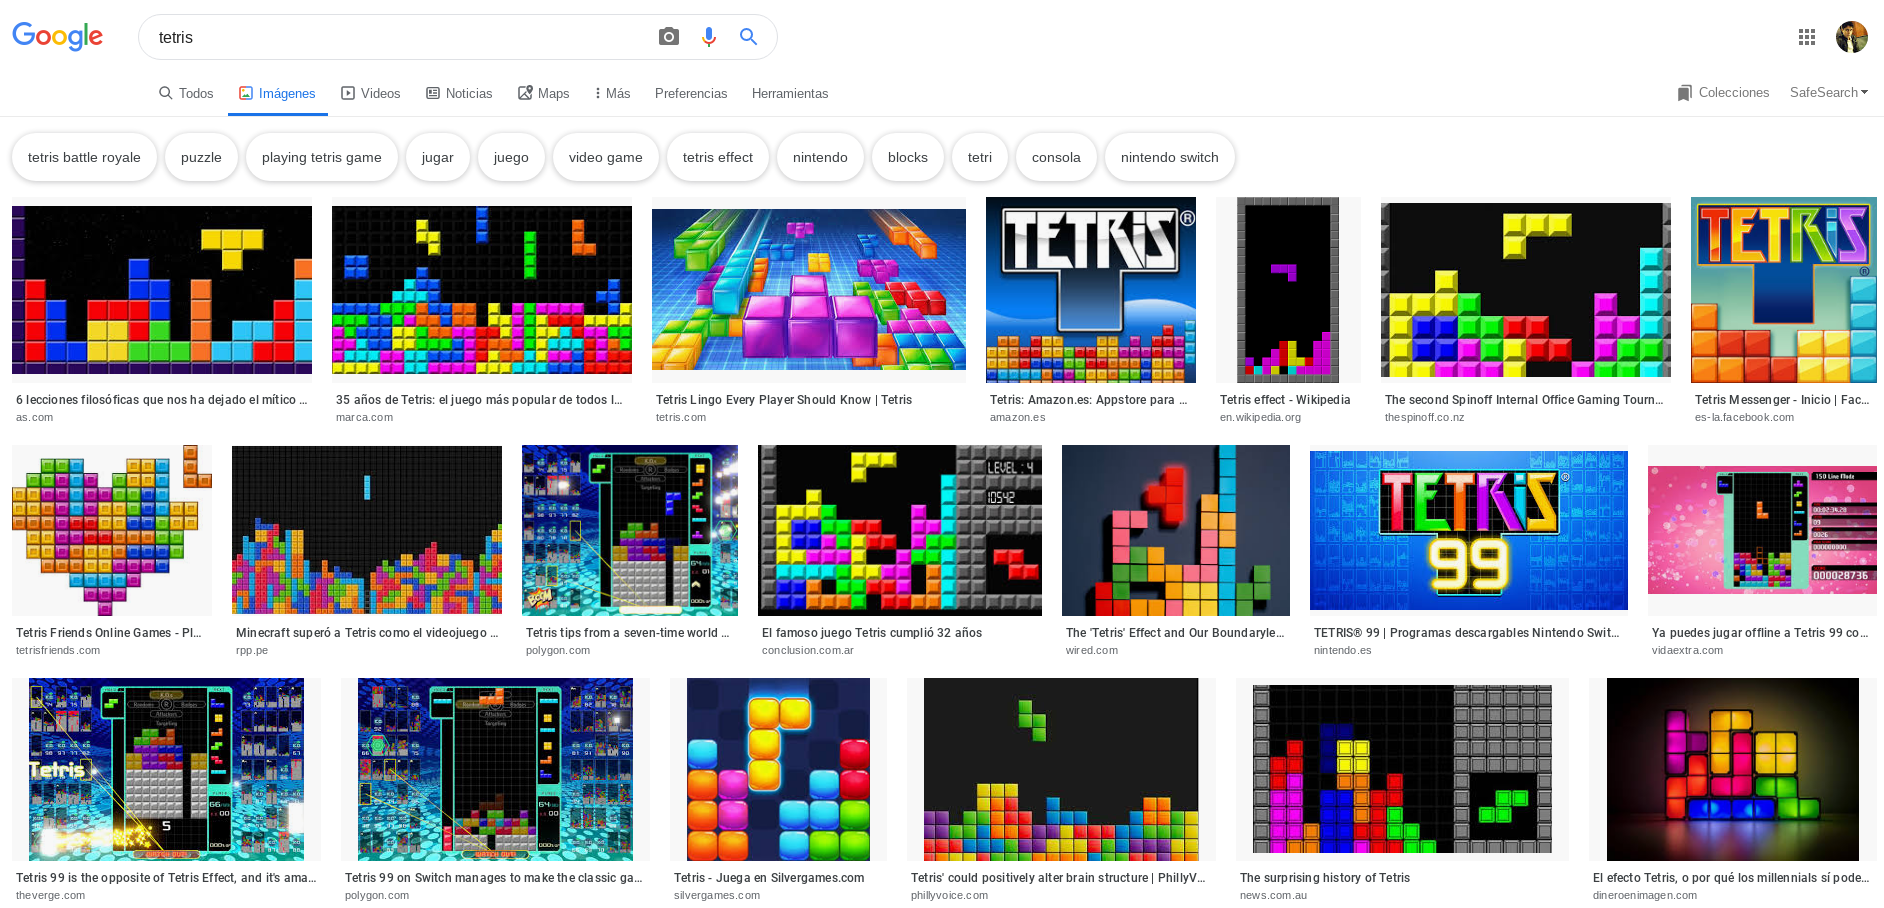
\includegraphics[scale=0.15]{./images/tetris_search.png}
\caption{Búsqueda de imágenes de Tetris en Google.}
\end{figure}

\end{frame} 

\begin{frame}
\frametitle{Tetris en la ciencia}

\begin{columns}
\column{0.5\textwidth}
Tetris es un problema ampliamente estudiado por la comunidad científica en distintas áreas: 

\begin{itemize}

\item Psicología
\item Matemáticas
\item Termodinámica
\item Ciencias de la Computación{\onslide<2->}:
\begin{itemize}

\item ¿Existe una estrategia para jugar en un tiempo indeterminado? 
\item ¿Cuál es la mejor estrategia de juego?
\item \textcolor<3->{red}{¿Existe alguna manera eficiente y automatizada de jugar Tetris?}
\item[] 

\end{itemize}
{\onslide}
\end{itemize}

\column{0.5\textwidth}
\begin{figure}
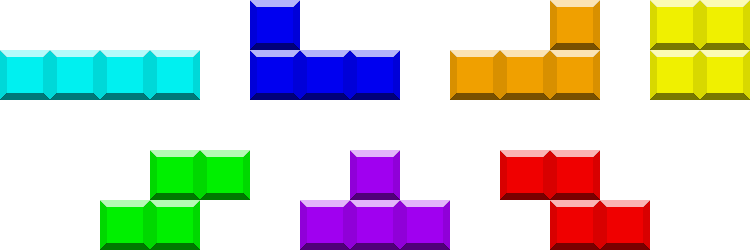
\includegraphics[scale=0.4]{./images/tetrominos.pdf}
\caption{Las piezas de Tetris.}
\end{figure}
\end{columns}


\end{frame}